\documentclass[a4paper]{article}
%\usepackage[affil-it]{authblk}
%\usepackage[backend=bibtex]{biblatex}
\usepackage{float}
\usepackage{amsmath}
\usepackage{geometry}
\usepackage{graphicx}
\usepackage{caption}
\usepackage{amssymb}
\usepackage{booktabs}
\usepackage[utf8]{inputenc}

\geometry{margin=1.5cm, vmargin={0pt,1cm}}
\setlength{\topmargin}{-1cm}
\setlength{\paperheight}{29.7cm}
\setlength{\textheight}{25.3cm}

\newcommand{\ProgramOutput}[1]{%
  \CatchFileDef{\ProgramOutputContent}{#1}{\endlinechar=-1 }%
  \begin{verbatim}
  \ProgramOutputContent
  \end{verbatim}
}

\begin{document}
% ==================================================
\title{Numerical Analysis Programming}

\author{Luo Kaicheng 3220103383
  \thanks{Electronic address: \texttt{3220103383@zju.edu.com}}}
%\affil{(Information and Computational Science 2201), Zhejiang University}

\date{Due time: \today}

\maketitle

\begin{abstract}
    Solutions to programming assignments.
\end{abstract}

% ============================================
\section*{Design Document}
The design revolves around two splines, \texttt{ppForm} and \texttt{BSpline}, for which two base classes \texttt{src/ppForm\_a\_BSpline/BSpline.hpp} and \texttt{src/ppForm\_a\_BSpline/ppForm.hpp} have been designed. In reality, these two base classes implement spline calculations of any order, knots, and arbitrary boundary conditions, using JSON as the control input.

\subsection*{How to Use the Program}

The base class requires the following JSON input:

\begin{verbatim}
{
    "dimension": 1,
    "order": 3,
    "boundary condition": {
        "equals": [],
        "values": [[0,1,2,3],[0,0,0,0],[[1],[2],[3],[4]]],
        "exists": [2,1]
    },
    "data points": [0.0, 2.0, 4.0, 9.0],
    "range": {
        "end": 10,
        "begin": 0
    }
}
\end{verbatim}

- \texttt{dimension} is the input dimension.
- \texttt{order} is the order of the spline.
- \texttt{data points} refer to the values of $t_i$, i.e., the knots.
- \texttt{range} indicates the required range, controlled by \texttt{begin} and \texttt{end}.

\subsubsection*{Boundary Condition}

\texttt{boundary condition} is an additional condition that supports any mix and free combination, including three types:

\begin{itemize}
    \item \texttt{"equals"}: An array \([knot1, order1, knot2, order2]\), which contains four arrays \texttt{knot1}, \texttt{order1}, \texttt{knot2}, \texttt{order2}. The elements at the same index in the four arrays are read in sequence to form equations. For example, if \texttt{list1}=[0, 1], \texttt{order1}=[1, 2], \texttt{list2}=[2, 3], \texttt{order2}=[2, 3], then the first element of the four arrays is read in sequence to form equations, the 1st-order derivative at the 0th node is equal to the 2nd-order derivative at the 2nd node. And so on.
    \item \texttt{"values"}: Represents specific values, composed of arrays \([knot1, order1, value]\), the first two store the point order and derivative order, and the third stores the corresponding derivative value. Considering high-dimensional problems, \texttt{value} is required to be a two-dimensional array, for example \([ [1, 2], [2, 3], [3, 4] ]\), representing the first derivative value is the vector \((1, 2)\), the second derivative value is \((2, 3)\), and so on. Note that even if the output is 1-dimensional, it should also be represented as a two-dimensional array for unified management, for example \(f''(t_0) = 0, f''(t_n) = 0\) is represented as \([ [0, n], [2, 2], [[0], [0]] ]\).
    \item \texttt{"exists"}: A one-dimensional array, indicating the existence of the highest-order derivative at certain nodes, in the form of \([a, b, \dots]\), indicating that the highest-order derivative exists at nodes \(a, b, \dots\). Note that the two edge points cannot be selected because their highest-order derivatives are known.
\end{itemize}

From these two base classes, it is very easy to control the input and output, inherit and implement five boundary condition spline subclasses. Moreover, the base classes themselves are more flexible.

\subsection*{Base Class Implementation Method}

Next, the implementation methods of these two base classes are introduced.

ppForm: First, read all JSON information into private variables, then scale each knot so that the average value of the intervals is 1, otherwise it will cause a large numerical calculation error in the subsequent process. In fact, the fitted function is \(f(t) = S(at)\), where \(a\) is the average interval previously. Similarly, for the derivative values, they should also be scaled, multiplied by the power of \(a\), and the order is the order of the derivative. In this way, when the fitted function is input \(t\) later, only \(f(t/a) = S(t)\) needs to be calculated.

When calculating the coefficients of each interval, we process each dimension so that each dimension corresponds to a set of different coefficients. The function values, derivative values, and other equation conditions corresponding to each dimension are input into the corresponding functions in the file \texttt{src/ppForm\_a\_BSpline/ppForm\_options} to obtain the coefficients corresponding to each interval.

Here, three calculation methods, version 1, version 2, and version 3, are implemented. You can specify the version by inputting 1, 2, or 3 in the constructor of \texttt{ppForm} (ppForm(json j,int version=1);), and the default version is 1.

\subsection*{version3}

Each unknown element can be represented by a vector, and then each vector is recursively calculated to obtain the vector representation of all coefficients. We initially assume that the unknowns are \((f_0, f_1, \dots, f_{N-1}, m_1/1, m_2/2, \dots, m_{n-1}/(n-1)!)\), where \(f_i\) corresponds to the function value at the \(i\)th point, and \(m_i\) represents the \(i\)th-order derivative value of the first node. It is assumed that all are unknowns at the beginning, and there are \(N+n-1\) unknowns in total.

It is easy to know that the coefficients of the first interval can be represented by the combination of \((f_0, f_1, \dots, f_{N-1}, m_1/1, m_2/2, \dots, m_{n-1}/(n-1)!)\). Let the first interval be
\[
\Sigma_{i=0}^{n} a_i (x - t_0)^i
\]
When \(i \neq n\), \(a_i = (0, 0, \dots, 1, \dots, 0, 0, \dots) \times (f_0, f_1, \dots, f_{N-1}, m_1/1, m_2/2, \dots, m_{n-1}/(n-1)!)^T\), where the position of 1 corresponds to the position of \(m_i/i!\).

When \(i = n\), using the Hermite interpolation formula,
\[
a_n = \frac{\frac{f_1 - f_0}{t_1 - t_0} - \frac{m_1}{1}}{(t_1 - t_0)} - \dots
\]
Also composed of unknowns \((f_0, f_1, \dots, f_{N-1}, m_1/1, m_2/2, \dots, m_{n-1}/(n-1)!)\).

In this way, we get
\[
\begin{pmatrix}
a_0 & a_1 & \dots & a_n
\end{pmatrix}
=
\begin{pmatrix}
1 & 0 & 0 & 0 & \dots & 0 \\
0 & 0 & \dots & 1 & 0 & \dots \\
0 & 0 & \dots & 0 & 1 & \dots \\
\vdots & \frac{-1}{(t_1 - t_0)^n} & \dots & \vdots
\end{pmatrix}
(f_0, f_1, \dots, f_{N-1}, m_1/1, m_2/2, \dots, m_{n-1}/(n-1)!)^T
\]

From this coefficient matrix, we can deduce the coefficient matrix of all intervals about \((f_0, f_1, \dots, f_{N-1}, m_1/1, m_2/2, \dots, m_{n-1}/(n-1)!)^T\).

From the coefficients of the previous interval to the derivatives at the right
endpoint
\[
\delta = t_i - t_{i-1}
\]
\[
(f'(t_i), f''(t_i), \dots, f^{n-1}(t_i))^T
=
\begin{pmatrix}
1 & 2\delta & \dots & n\delta^{n-1} \\
0 & 2 & \dots & n(n-1)\delta^{n-2} \\
\vdots & \vdots & \dots & n! \delta
\end{pmatrix}
(a_1, a_2, \dots, a_n)^T
\]

From the endpoint derivatives to the coefficients of this interval
\[
\delta = t_{i+1} - t_{i}
\]
\[
(a'_1, a'_2, \dots, a'_n)^T
=
\begin{pmatrix}
\frac{1}{1!} & 0 & \dots & 0 \\
0 & \frac{1}{2!} & \dots & 0 \\
\vdots & \vdots & \dots & \frac{1}{(n-1)!} \\
-\frac{1}{\delta^{n-1}} & 0 & \dots & n! \delta \dots & -\frac{1}{(n-1)! \delta}
\end{pmatrix}
(f'(t_i), f''(t_i), \dots, f^{n-1}(t_i))^T
+ (0, 0, \dots, \frac{f(x_{i+1})}{\delta^n})^T
\]

In this way, we get all the coefficients of the intervals, and the coefficients of the derivatives at the points about \((f_0, f_1, \dots, f_{N-1}, m_1/1, m_2/2, \dots, m_{n-1}/(n-1)!)^T\).

At this time, we can extract the corresponding equations from the provided conditions to form a matrix for solving. Construct an \(m \times k\) matrix and an \(m \times 1\) vector, where \(m\) is the number of all provided conditions, each row corresponds to a condition; \(k\) is \(n + N - 1\).

If it is a condition that provides specific values (\texttt{values}), fill in the corresponding coefficient row of the corresponding point's corresponding derivative order, and fill in the corresponding value in the vector position. If it is a condition that provides equality (\texttt{equals}), subtract the corresponding coefficient row of the two corresponding points' corresponding derivative orders and fill in, and fill 0 in the vector position. If it is a condition that provides existence (\texttt{exists}), it means that the highest-order term coefficients of the two adjacent intervals are equal, subtract the two corresponding coefficient rows and fill in, and fill 0 in the vector position.

Use Eigen3 to solve, and get the solution \((f_0, f_1, \dots, f_{N-1}, m_1/1, m_2/2, \dots, m_{n-1}/(n-1)!)^T\) of the specific values. Then, through matrix multiplication, it is easy to calculate the coefficients of each interval. It should be noted that the obtained coefficients are the coefficients of Hermite interpolation, and when calculating, the left endpoint \(t_i\) should be subtracted, and then brought into the polynomial.

\subsection*{version2}

The implementation method of version 2 is similar to version 3, with the difference being that it takes into account that most splines will provide the function values of $n$ knots, and periodic boundary conditions will also provide $n-1$. Therefore, a separate version is designed for cases where at least the first $n-1$ nodes have specific function values. The rest of the implementation is the same as version 3, except that the 0th-order derivative values of the first $n-1$ points are treated as constants.

Considering the coefficients of all intervals, the coefficients of node derivatives with respect to $(1, f_n, m_1/1, m_2/2, \dots, m_{n-1}/(n-1)!)$, where 1 represents the constant term, and $f_n$ is the function value of the $n$th node. This can significantly reduce the size of the solution matrix to $n + 1$.

\subsection*{version1}

It is observed that in the calculations of the first two methods, coefficients are recorded throughout, and a large number of combinations are multiplied during the recursion process. When the number of knots is small, the first two methods are very accurate.

However, it is observed that when the number of intervals is very large, i.e., when there are many sampling points, the coefficients for the last interval tend to inflate significantly, such as to the order of 1e30, which can lead to very large errors in subsequent calculations.

For example, if the original solution is $(x_1,x_2)=(1,1)$, there might be equations of the form $1e30 \cdot x_1 - (1e30 - 1) \cdot x_2 = 1$.

In contrast, B-splines do not use recursion and the weight of each coefficient in the equations is close, leading to better matrix properties and avoiding such situations.

Therefore, version 1 is constructed in a manner similar to B-splines. The coefficients of the intervals are taken as unknowns, and the continuity conditions of the intermediate knots are also included in the equations, rather than using recursion.

\begin{verbatim}
for (int t=1; t < N-1; t++)
{
    int starting_line_index=(t-1)*(order);
    for (int j = 0; j < order; j++)
    {
        //Express the derivative of each point using the coefficients of the previous and next intervals
        add_differential_coefficients(matrix, starting_line_index + j, order, input_knots, t, j, 1);
        matrix(starting_line_index + j, (order + 1) * t + j) = -factorial(j);
    }
}
\end{verbatim}

This construct results in a larger equation size and is more time-consuming to solve, but it is more accurate.\\
\textbf{BSpline}
The interface part of the hpp is almost identical to ppForm. Read all JSON information into private variables, then scale each knot. Process each dimension separately so that each dimension corresponds to a set of different coefficients. Input the function values, derivative values, and other equation conditions corresponding to each dimension into the corresponding functions in the file \texttt{src/ppForm\_a\_BSpline/BSpline\_options} to obtain the coefficients corresponding to each dimension.

The coefficient solving part of BSpline is designed with only one version, which tabulates for each node to calculate the size of $B^n_{i}$ at this node. The obtained table can also be used for subsequent calculations of derivatives of various orders.

First, tabulate for each node $t_i$. Since $B_i$ spline is defined on $(t_{i-1},t_i)$, only $B_k$ with $k$ less than or equal to $i$ needs to be considered.
\[
\begin{pmatrix}
B^0_{2-n}(t_i) & B^0_{3-n}(t_i) & B^0_{4-n}(t_i) & \dots & B^0_{i}(t_i) \\
B^1_{2-n}(t_i) & B^1_{3-n}(t_i) & B^1_{4-n}(t_i) & \dots & B^1_{i}(t_i) \\
B^2_{2-n}(t_i) & B^2_{3-n}(t_i) & B^2_{4-n}(t_i) & \dots & B^2_{i}(t_i) \\
\vdots & \vdots & \vdots & \ddots & \vdots \\
B^n_{2-n}(t_i) & B^n_{3-n}(t_i) & B^n_{4-n}(t_i) & \dots & B^n_{i}(t_i)
\end{pmatrix}
\]

The update method is as follows:
\begin{verbatim}
// Update the current layer using the recursive formula
vector<double> update_B(vector<double> B, vector<double> knots, int current_order, double x) {
    for (int k = max(0, B.size() - 2 - current_order); k <= (int)B.size() - 2; k++) {
        B[k] = B[k] * (x - get_ti(k - 1, knots)) / (get_ti(current_order + k, knots) - get_ti(k - 1, knots)) +
               B[k + 1] * (get_ti(k + current_order + 1, knots) - x) / (get_ti(current_order + k + 1, knots) - get_ti(k, knots));
    }
    B[B.size() - 1] *= (x - get_ti(B.size() - 2, knots)) / (get_ti(current_order + B.size() - 1, knots) - get_ti(B.size() - 2, knots));
    return B;
}

// Construct the value table
vector<vector<double>> construct_value_table(vector<double> knots, int order, int index, double x) {
    vector<vector<double>> table = {};
    vector<double> B(index + 1, 0); // Note that the index here is the index after adding 2-n to 0, these arbitrarily designated nodes
    B[index] = 1;
    table.push_back(B);
    for (int i = 0; i < order; i++) {
        table.push_back(update_B(table[table.size() - 1], knots, i, x));
    }
    return table;
}
\end{verbatim}

After tabulating for all nodes in the interval, if the derivative information at a certain point is needed, it can be calculated using the function value table $B\_value$ at that point.

Given the coefficient matrix
\[ A = \text{coefficients} = \begin{bmatrix}
1 & 0 & 0 & \cdots & 0 \\
0 & 1 & 0 & \cdots & 0 \\
0 & 0 & 1 & \cdots & 0 \\
\vdots & \vdots & \vdots & \ddots & \vdots \\
0 & 0 & 0 & \cdots & 1
\end{bmatrix} \]
as the identity matrix, and the 0th-order derivative $(B^n_{2-n}(t_i) , B^n_{3-n}(t_i) , B^n_{4-n}(t_i) , \dots , B^n_{i}(t_i)) = B\_value.row(n) * A$.

\[ (B'^n_{2-n}(t_i) , B'^n_{3-n}(t_i) , B'^n_{4-n}(t_i) , \dots , B'^n_{i}(t_i)) = \left(\frac{nB_k^{n-1}(t_i)}{t_{k+n-1}-t_{k-1}} - \frac{nB_{k+1}^{n-1}(t_i)}{t_{k+n}-t_{k}}\right) = B\_value.row(n-1) * BA \]

where
\[ B = \begin{bmatrix}
\frac{\text{order}-i}{t_{0+order-i-1} - t_{0-1}} & -\frac{\text{order}-i}{t_{1+order-i-1} - t_{1-1}} & 0 & \cdots & 0 \\
0 & \frac{\text{order}-i}{t_{1+order-i-1} - t_{1-1}} & -\frac{\text{order}-i}{t_{2+order-i-1} - t_{2-1}} & \cdots & 0 \\
0 & 0 & \frac{\text{order}-i}{t_{2+order-i-1} - t_{2-1}} & \cdots & 0 \\
\vdots & \vdots & \vdots & \ddots & \vdots \\
0 & 0 & 0 & \cdots & \frac{\text{order}-i}{t_{\text{index}+order-i-1} - t_{\text{index}-1}}
\end{bmatrix} \]

Let $A = BA$, update the iteration, and you can get the 0-n-1th order derivatives of 
$(B^n_{2-n}(x) , B^n_{3-n}(x) , B^n_{4-n}(x) , \dots , B^n_{i}(x))$ at $t_i$.

In fact, by using the method of only considering the left-hand side derivative, you can calculate the nth derivative n times. The calculation code is as follows.

\begin{verbatim}
    vector<vector<double>> construct_derivatives_table(vector<vector<double>> value_table,vector<double> knots){
        vector<vector<double>> difftable;
        int order=value_table.size()-1;
        int index=value_table[0].size()-1;
        Eigen::MatrixXd matrix=Eigen::MatrixXd::Zero(index+1, index+1);
        Eigen::MatrixXd coefficients=Eigen::MatrixXd::Identity(index+1, index+1);     
        difftable.push_back(value_table[order]);//0_th dirivation
        for (int i = 0; i < order; i++)
        {
            Eigen::MatrixXd values(1,index+1);
            values.row(0)=Eigen::Map<const Eigen::VectorXd>(value_table[order-i-1].data(),index+1);
            for (int j = 0; j < index+1; j++)
            {
                matrix(j,j)=(double)(order-i)/(get_ti(j+order-i-1,knots)-get_ti(j-1,knots));
                if(j<index) matrix(j+1,j)=-(double)(order-i)/(get_ti(j+order-i,knots)-get_ti(j,knots));
            }
            coefficients=matrix*coefficients;
            Eigen::MatrixXd deriv=values*coefficients;
            vector<double> result(deriv.data(), deriv.data() + deriv.rows() * deriv.cols());
            difftable.push_back(result);
        }
        return difftable;
}
\end{verbatim}
At this point, we can extract the corresponding equations from the provided conditions to form a matrix for solving. Construct an $m \times k$ matrix and an $m \times 1$ vector, where $m$ is the number of all provided conditions, each row corresponding to a condition; $k$ is $n + N - 1$.

\[
S(t) = \sum_{i=2-n}^{N} a_i B_i^n(t) \in \mathbb{R}
\]
\[
S(t)^{(n)} = \sum_{i=2-n}^{N} a_i B_i^n(t)^{(n)} \in \mathbb{R}
\]

If it is a condition that provides specific values (\texttt{values}), fill in the corresponding $B_k^n(t)^{(n)}(t_i)$ (including $n=0$) for the corresponding point and fill in the corresponding value in the vector position. If it is a condition that provides equality (\texttt{equals}), subtract the corresponding $B_k^n(t)^{(n)}(t_i)$ of the two corresponding points and fill in, and put 0 in the vector position. If it is a condition that provides existence (\texttt{exists}), when constructing the derivative matrix earlier, it is possible to consider the left $n$-th derivative of the point and the left $n$-th derivative of the next interval, both sides of the $n$-th derivative should be constants and equal, fill in similarly.

Thus, all coefficients $a_i$ can be solved to obtain the curve.

When outputting points, it is similar to the construction process, just bring in the previously constructed value table.\\

\section*{Problem 1}
Input template reference \texttt{src/problems\_1\_7/problem1/config.json}.
Location \texttt{src/problems\_1\_7/problem1}
Use two subclasses to control the input and output formats of the base class.

\begin{verbatim}
class BSpline_1_0: public BSpline {
private:
    vector<double> knots; 
    double start, end;
public:
    BSpline_1_0(json j): BSpline(j) {
        if (!j["data points"].is_null()) {
            knots = j["data points"].get<vector<double>>();
            if (knots.empty() || knots.size() < 2) {
                cout << "Inadequate knots" << endl;
                throw "Inadequate datapoints";
            }
        } else {
            cout << "No datapoints" << endl;
            throw "No datapoints";
        }
        
        if (!j["range"]["begin"].is_null()) start = j["range"]["begin"];
        else start = knots[0];
        if (!j["range"]["end"].is_null()) end = j["range"]["end"];
        else end = knots[knots.size()-1];
    };
    double get_value(double t) {
        return BSpline::get_value(t)[0];
    }
};

and

class ppform_1_0: public ppForm {
private:
    vector<double> knots;
    double start, end;
public:
    ppform_1_0(json j): ppForm(j) {
        if (!j["data points"].is_null()) {
            knots = j["data points"].get<vector<double>>();
            if (knots.empty() || knots.size() < 2) {
                cout << "Inadequate knots" << endl;
                throw "Inadequate datapoints";
            }
        } else {
            cout << "No datapoints" << endl;
            throw "No datapoints";
        }
        
        if (!j["range"]["begin"].is_null()) start = j["range"]["begin"];
        else start = knots[0];
        if (!j["range"]["end"].is_null()) end = j["range"]["end"];
        else end = knots[knots.size()-1];
    };
    double get_value(double t) {
        return ppForm::get_value(t)[0];
    }
};
\end{verbatim}

Input points to the base class and specify the output as one-dimensional.
Plot results:

\begin{figure}[H] 
    \centering
    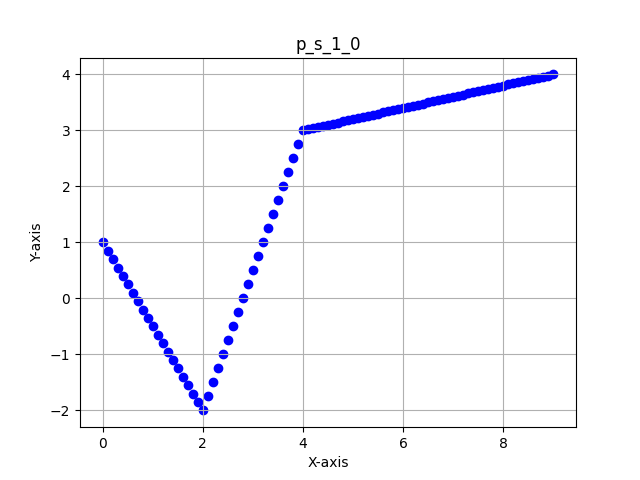
\includegraphics{../figure/p_s_1_0.png}
    \caption{P1\_ppform}
\end{figure}

\begin{figure}[H] 
    \centering
    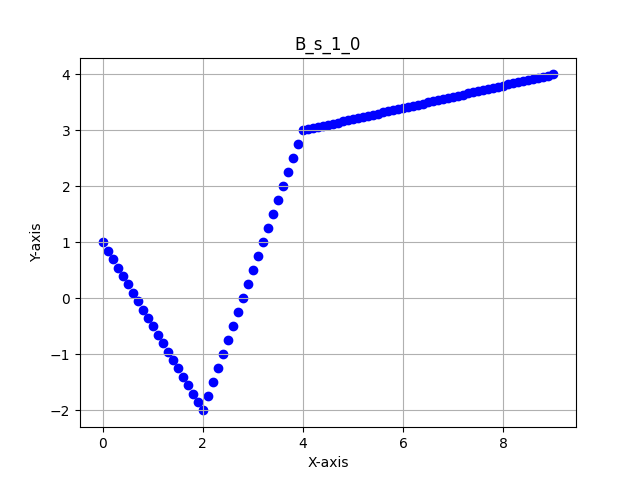
\includegraphics{../figure/B_s_1_0.png}
    \caption{P1\_BSpline}
\end{figure}

\section*{Problem 2}
Similar to the first problem, this problem implements control over five types of boundary conditions, all of which are standardized by subclasses to input the JSON format to the base class.
The problem is located at: \texttt{src/problems\_1\_7/problem2}
Template reference: \texttt{src/problem\_1\_7/problem2/config.json}

\begin{verbatim}
{
    "dimension": 1,
    "order": 3,
    "boundary condition": "natural",
    "derivation": [],
    "data points": [0.0, 2.0, 4.0, 9.0],
    "function values": [1,3,5,7],
    "range": {
        "end": 9,
        "begin": 0
    }
}
\end{verbatim}

A main function is used to select the boundary condition to be used. Each file(.hpp) involves transforming conditions such as "natural," "complete," etc., into their corresponding forms of "values," "equals," and "exists," constructing a new JSON to be passed into the base class.
Detailed code can be found in:
"\texttt{ppform\_2\_3\_periodic.hpp}"
"\texttt{ppform\_2\_3\_complete.hpp}"
"\texttt{ppform\_2\_3\_natural.hpp}"
"\texttt{ppform\_2\_3\_not\_a\_knot.hpp}"
"\texttt{ppform\_2\_3\_specific\_2\_deri.hpp}"

Test case plot results:

\begin{figure}[H] 
    \centering
    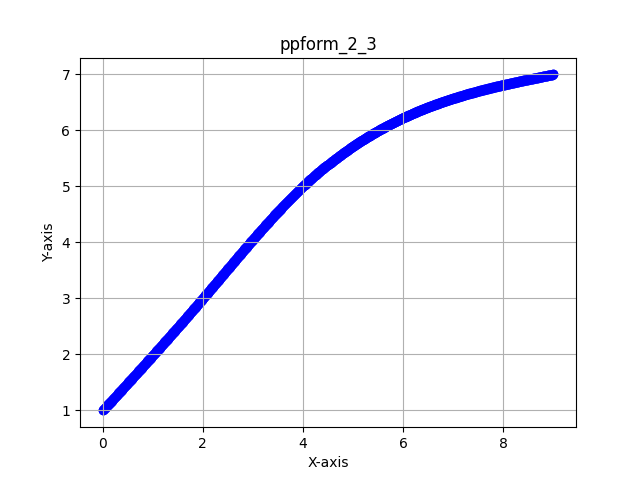
\includegraphics{../figure/ppform_2_3.png} 
    \caption{ppform\_2\_3} 
\end{figure}

\section*{Problem 3}
Almost identical to the second problem, the base class passed in is changed to BSpline. Other implementation methods are the same, and it also implements control over five types of boundary conditions.
The problem is located at: \texttt{src/problems\_1\_7/problem3}
Template reference: \texttt{src/problem\_1\_7/problem3/config.json}
The template is the same as Problem 2.
Similarly, a main function is used to select the boundary condition to be used, transforming conditions such as "natural," "complete," etc., into their corresponding forms of "values," "equals," and "exists," constructing a new JSON to be passed into the base class.
Detailed code can be found in:
"\texttt{BSpline\_2\_3\_periodic.hpp}"
"\texttt{BSpline\_2\_3\_complete.hpp}"
"\texttt{BSpline\_2\_3\_natural.hpp}"
"\texttt{BSpline\_2\_3\_not\_a\_knot.hpp}"
"\texttt{BSpline\_2\_3\_specific\_2\_deri.hpp}"
Test case plot results:
\begin{figure}[H] 
    \centering
    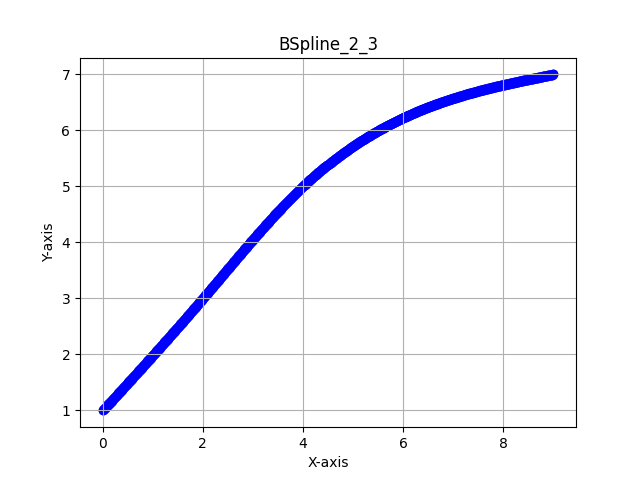
\includegraphics{../figure/BSpline_2_3.png} 
    \caption{BSpline\_2\_3} 
\end{figure}
However, considering the Theorem required in Problem C, a different implementation scheme is used, see Problem C later in the document.

\section*{Problem 4}
The problem is located at: \texttt{src/problems\_1\_7/problem4}
Template reference: \texttt{src/problem\_1\_7/problem4/config.json}
Directly call the base class function, a test case is selected, and the image is plotted.
\begin{figure}[H] 
    \centering
    \includegraphics{../figure/compare_B.png} 
    \caption{compare B} 
\end{figure}

\begin{figure}[H] 
    \centering
    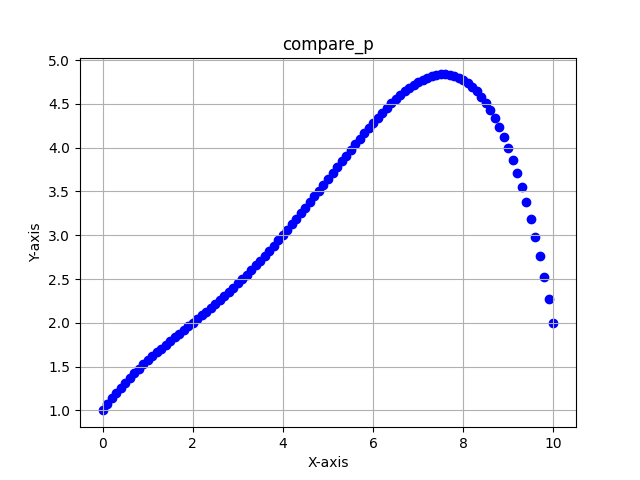
\includegraphics{../figure/compare_p.png} 
    \caption{compare p} 
\end{figure}
Directly compare the output data points, and it can be seen that the results are the same.
B:
\begin{verbatim}
0 1
0.1 1.07002
0.2 1.13648
0.3 1.19965
0.4 1.25979
0.5 1.31719
0.6 1.37208
0.7 1.42472
0.8 1.47534
0.9 1.52417
\dots
\end{verbatim}
p:
\begin{verbatim}
0 1
0.1 1.07002
0.2 1.13648
0.3 1.19965
0.4 1.25979
0.5 1.31719
0.6 1.37208
0.7 1.42472
0.8 1.47534
0.9 1.52417
\dots
\end{verbatim}

\section*{Problem 5}
The problem is located at: \texttt{src/problems\_1\_7/problem5}
Template reference: \texttt{src/problem\_1\_7/problem5/config.json}
When coefficients are directly provided, we use JSON to record the coefficients, such as
\begin{verbatim}
{
    "dimension": 1,
    "order": 3,
    "coefficients": [[1,-1,3,4,7,2]],
    "data points": [0.0, 2.0, 4.0,9.0],
    "range": {
        "end": 9,
        "begin": 0
    }
}
\end{verbatim}
Note that the size of coefficients should be the size of data points plus order-1.
Here, the base class function for constructing the value table is directly called.
\begin{verbatim}
// Update the current layer using the recursive formula
vector<double> update_B(vector<double> B, vector<double> knots, int current_order, double x) {
    for (int k = max(0, B.size() - 2 - current_order); k <= (int)B.size() - 2; k++) {
        B[k] = B[k] * (x - get_ti(k - 1, knots)) / (get_ti(current_order + k, knots) - get_ti(k - 1, knots)) +
               B[k + 1] * (get_ti(k + current_order + 1, knots) - x) / (get_ti(current_order + k + 1, knots) - get_ti(k, knots));
    }
    B[B.size() - 1] *= (x - get_ti(B.size() - 2, knots)) / (get_ti(current_order + B.size() - 1, knots) - get_ti(B.size() - 2, knots));
    return B;
}

// Construct the value table
vector<vector<double>> construct_value_table(vector<double> knots, int order, int index, double x) {
    vector<vector<double>> table = {};
    vector<double> B(index + 1, 0); // Note that the index here is the index after adding 2-n to 0, these arbitrarily designated nodes
    B[index] = 1;
    table.push_back(B);
    for (int i = 0; i < order; i++) {
        table.push_back(update_B(table[table.size() - 1], knots, i, x));
    }
    return table;
}
\end{verbatim}
Calculate the value of each $B^n_k(x)$ at the current point layer by layer, and finally multiply by the coefficients to sum up.
Example result:
\begin{figure}[H] 
    \centering
    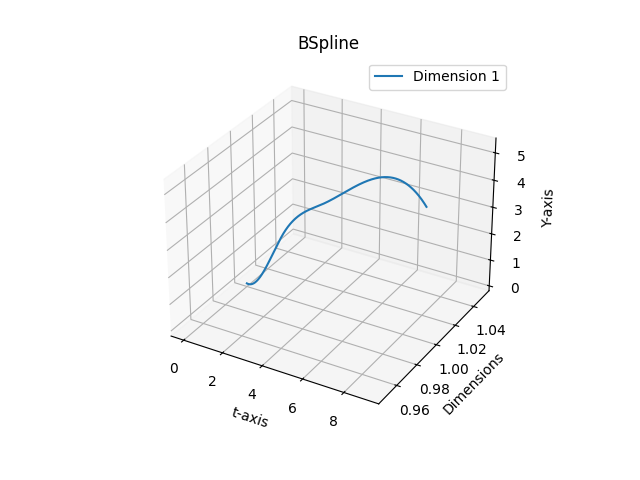
\includegraphics{../figure/BSpline.png} 
    \caption{BSpline} 
\end{figure}
\section*{Problem 6}
Implement spline curve fitting on a plane, providing two methods using ppForm and BSpline.
The fitting header files are located in \texttt{src/Curving\_fit/plane}.
The test files are located in \texttt{src/problems\_1\_7/problem6}.
The template is in \texttt{src/problems\_1\_7/problem6/config.json}.

\begin{verbatim}
{
    "dimension":2,
    "order": 3,
    "boundary condition": {
        "equals": [],
        "values": [],
        "exists": [1,2]
    },
    "points": 
        [[0,2],[ 2,7],[ 4,4],[9,10]],
    "range":{
        "begin":0,
        "end":1
    }
}
\end{verbatim}

This template is for plane function fitting, where "points" are the control points. The "range" does not need to be set manually, as it is the range of the parameter during parameterization and does not affect the results.
"Boundary condition" can also be set arbitrarily, as different boundary conditions will correspond to different fitting effects.
The structure's constructor \texttt{curve\_fitting\_B(json j, string sampling\_mode="equal")}, \texttt{curve\_fitting\_p(json j, string sampling\_mode="equal")} accepts JSON and two parameters of parameterization methods.
Parameterization methods can be chosen as "equal" or "Chord".

The specific implementation still involves reading the JSON content and converting it into a JSON that can be used by the base classes BSpline and ppForm.
However, the nodes are selected by oneself, and two selection methods are provided here, equal distance or cumulative chord length.

The sampling methods are as follows:
\begin{verbatim}
    if(sampling_mode=="equal"){
        for (int i = 0; i < N; ++i) {
            double t = static_cast<double>(i) / (N - 1); 
            knots.push_back((end-start)*t+start);
        }
    }else if(sampling_mode=="Chord"){
        vector<double> chord={0};
        for (size_t i = 1; i <points.size(); i++)//Calculate the cumulative chord length
        {
            double len=0;
            for (size_t j = 0; j < points[i].size(); j++) len+=(points[i][j]-points[i-1][j])*(points[i][j]-points[i-1][j]);
            len=sqrt(len)+chord[chord.size()-1];
            chord.push_back(len);
        }
        for (size_t i = 0; i < points.size(); i++)
        {
            knots.push_back((end-start)*chord[i]/chord[chord.size()-1]+start);
        }
    }else{
        cerr<<"no such sampling_mode"<<endl;
        throw "no such sampling_mode";
    }
\end{verbatim}

When fitting, points are taken by calling the base class's \texttt{get\_value} function, which returns the predicted value.

\begin{figure}[H] 
    \centering
    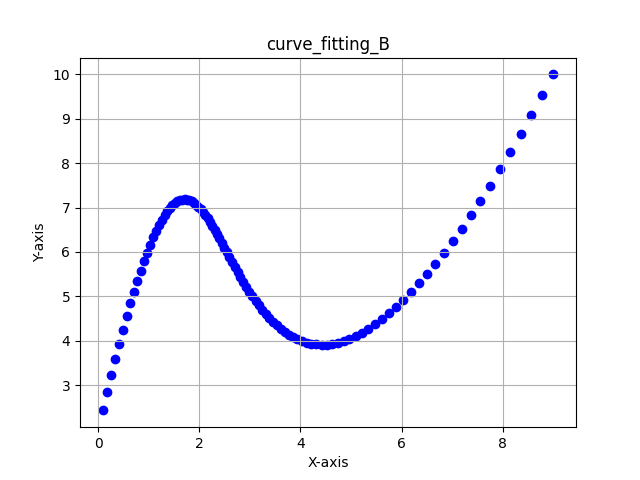
\includegraphics{../figure/curve_fitting_B.png} 
    \caption{curve\_fitting\_B} 
\end{figure}

\begin{figure}[H] 
    \centering
    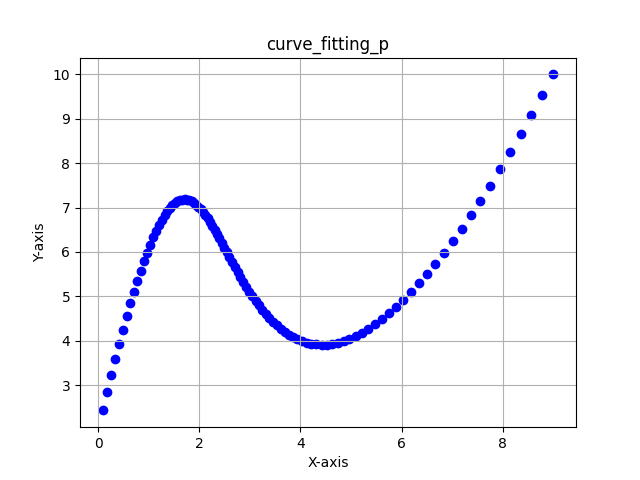
\includegraphics{../figure/curve_fitting_p.png} 
    \caption{curve\_fitting\_p} 
\end{figure}

Call the function to check for self-intersection, and it is determined that there is no self-intersection.
Problem E also uses these header files, see later in the document.

\section*{Problem 7}

The fitting header files are located in \texttt{src/Curving\_fit/sphere}.
The test files are located in \texttt{src/problems\_1\_7/problem7}.
The template is in \texttt{src/problems\_1\_7/problem7/config.json}.

\begin{verbatim}
{
    "boundary condition": {
        "exists": [
            1,
            98
        ]
    },
    "centre": [
        0.0,
        0.0,
        0.0
    ],
    "order": 3,
    "points": [
        [
            0.0,
            0.0,
            1.0
        ],
        [
            0.09549150281031595,
            0.04251555625300347,
            0.9945218953685862
        ],
        .....
    ],
    "radius": 1.0,
    "range": {
        "begin": 0,
        "end": 1
    }
}
\end{verbatim}

Arbitrarily specify boundary conditions, provide control points, center, radius, and other parameters.
Here, a spiral line generated in \texttt{src/problems\_1\_7/problem7/create\_test\_case.cpp} is used.

Design idea:
First, convert three-dimensional coordinates into two-dimensional coordinates using latitude and longitude parameterization.
Calculate two deflection angles.
Note that latitude can always change continuously within [-90,90], while longitude may experience a sudden change between 0 and 2 pi. To ensure the continuity of the drawing,
the longitude information of the previous point is saved here, and the longitude closest to the previous longitude is selected to ensure continuous change in longitude, and the domain of definition is expanded.

\begin{verbatim}
    while (1){
        if(fabs(angle2+2*pi-angle)<fabs(angle2-angle)){
            angle2+=2*pi;
            continue;
        }else if(fabs(angle2-2*pi-angle)<fabs(angle2-angle)){
            angle2-=2*pi;
            continue;
        }
        break;
    } 
\end{verbatim}

It can be easily proven that when there are enough sampling points, the parameterization of the sampling points is continuous.
Another problem that may arise is the sudden change in longitude when the curve passes through the North or South Pole:

Rotation is introduced here, and it is difficult for the curve to cover the entire plane, so random sampling points are taken, and neither the point nor its symmetric point about the origin is within the control points.
Then rotate, using this point as the new North Pole.
Interpolate on the new sphere.
The interpolation result is then multiplied by the inverse rotation matrix to get the final point.

\begin{verbatim}
    while (true) {
        random_point = generate_random_point_on_sphere();
        generate_rotate=random_point;
        symmetric_point = -random_point;

        random_point[0]=centre[0]+random_point[0]*r;
        random_point[1]=centre[1]+random_point[1]*r;
        random_point[2]=centre[2]+random_point[2]*r;
        symmetric_point[0]=centre[0]+symmetric_point[0]*r;
        symmetric_point[1]=centre[1]+symmetric_point[1]*r;
        symmetric_point[2]=centre[2]+symmetric_point[2]*r;
        // Check if the random point and its symmetric point are in dots
        if (!is_point_in_dots(random_point, dots) && !is_point_in_dots(symmetric_point, dots)) {
            break; // Found a suitable point, exit the loop
        }
    }
    Matrix3d rotation_matrix = get_rotation_matrix_to_north_pole(generate_rotate);
\end{verbatim}

For the derivative values, corresponding transformations are also needed. The derivative values in the three-dimensional image should be a three-element vector, and the derivative values corresponding to the two angles are calculated using the derivative rules.

\begin{verbatim}
    vector<double> process_derivation(vector<double> dots,vector<double> values, int order,double r,double rate,Matrix3d rotation_matrix){
        double coeff_11,coeff_21,coeff_22,coeff_31,coeff_32;
        Vector3d point(values[0], values[1] , values[2]);
        Vector3d rotated_point = rotation_matrix * point;
        values={rotated_point[0],rotated_point[1],rotated_point[2]};

        int sign=order%4<2 ? 1:-1;
        if(order%2==1) {
            coeff_11=cos(dots[0])*r*sign;
            coeff_32=cos(dots[1])*r*sign*cos(dots[0]);
        }
        else {
            coeff_11=sin(dots[0])*r*sign;
            coeff_32=sin(dots[1])*r*sign*cos(dots[0]);
        }
        if(order%4==1||order%4==2) sign=-1;
        else sign=1;
        if(order%2==0){
            coeff_21=cos(dots[0])*sign*r*cos(dots[1]);
            coeff_31=cos(dots[0])signrsin(dots[1]);
            coeff_22=cos(dots[1])rsigncos(dots[0]);
        }else{
            coeff_21=sin(dots[0])signrcos(dots[1]);
            coeff_31=sin(dots[0])signrsin(dots[1]);
            coeff_22=sin(dots[1])rsign*cos(dots[0]);
        }
            Eigen::MatrixXd matrix=Eigen::MatrixXd::Zero(3, 2);
            Eigen::VectorXd target(3);
            matrix(0,0)=coeff_11;
            matrix(1,0)=coeff_21;
            matrix(1,1)=coeff_22;
            matrix(2,0)=coeff_31;
            matrix(2,1)=coeff_32;
            target[0]=values[0]*rate;
            target[1]=values[1]*rate;
            target[2]=values[2]*rate;
            Eigen::FullPivLUEigen::MatrixXd lu_decomp(matrix);
            if(lu_decomp.rank()<2){
                cout<<"incorrect derivative input"<<endl;
                throw "incorrect derivative input";
            }
            Eigen::VectorXd solution = matrix.colPivHouseholderQr().solve(target);
            vector<double> result(solution.data(), solution.data() + solution.size());
            return result;
            }
    \end{verbatim}
            
    Import the base class to get the spline.
    When taking values, get the corresponding two angles from the base class, transform them into spherical coordinates, and then multiply by the inverse rotation matrix.
    Here, a spiral line is used as an example.\\
    target:\\
    \begin{figure}[H]
    \centering
    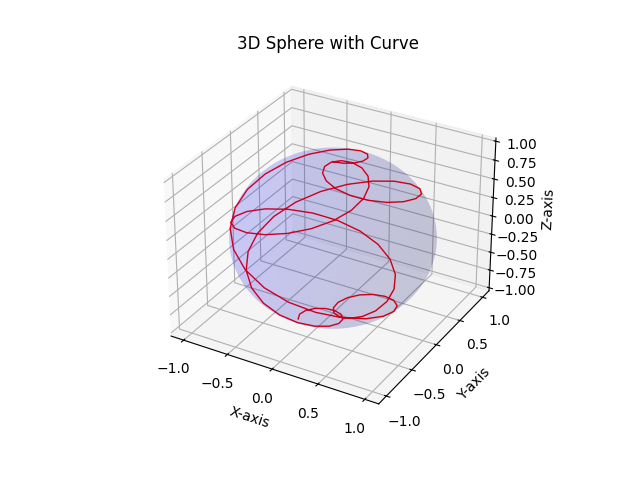
\includegraphics{../figure/3D Sphere with Curve.png}
    \caption{3D Sphere with Curve}
    \end{figure}
            
    \begin{figure}[H]
    \centering
    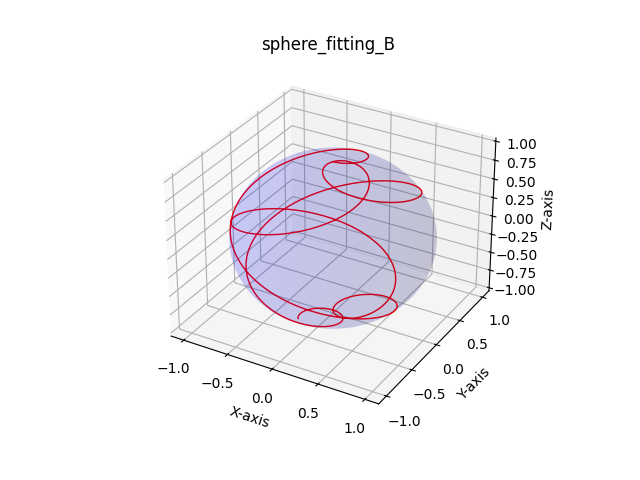
\includegraphics{../figure/sphere_fitting_B.png}
    \caption{sphere\_fitting\_B}
    \end{figure}
            
    \begin{figure}[H]
    \centering
    \includegraphics{../figure/sphere_fitting_P.png}
    \caption{sphere\_fitting\_P}
    \end{figure}

\section*{Problem A}
    The test file is located in \texttt{src/problems\_in\_chapter3/ProblemA.cpp}.
    
    Here, we take the natural spline of ppForm and BSpline as examples, construct JSON through uniform sampling, and run the calculation.
    ppForm:
    \begin{verbatim}
        vector<double> knots = construct(N, start, end);
        vector<double> f_values = construct_f(knots);
        json j = {
            {"dimension", 1},
            {"order", 3},
            {"boundary condition", "natural"},
            {"data points", knots},
            {"function values", f_values},
            {"range", {
                {"end", 1},
                {"begin", -1}
            }}
        };
        ppform_2_3_natural pp(j);
        double max_error = 0;
        for (size_t i = 0; i < knots.size() - 1; i++) {
            double result = pp.get_value((knots[i] + knots[i + 1]) / 2);
            double result2 = f((knots[i] + knots[i + 1]) / 2);
            if (abs(result2 - result) > max_error) max_error = abs(result2 - result);
        }
        return max_error;
    \end{verbatim}
    BSpline:
    \begin{verbatim}
        vector<double> knots = construct(N, start, end);
        vector<double> f_values = construct_f(knots);
        json j = {
            {"dimension", 1},
            {"order", 3},
            {"boundary condition", "natural"},
            {"data points", knots},
            {"function values", f_values},
            {"range", {
                {"end", 1},
                {"begin", -1}
            }}
        };
        BSpline_2_3_natural bs(j);
        double max_error = 0;
        for (size_t i = 0; i < knots.size() - 1; i++) {
            double result = bs.get_value((knots[i] + knots[i + 1]) / 2);
            double result2 = f((knots[i] + knots[i + 1]) / 2);
            if (abs(result2 - result) > max_error) max_error = abs(result2 - result);
        }
        return max_error;
    \end{verbatim}
    Plot the function image as the number of points increases.
    \begin{figure}[H] 
        \centering
        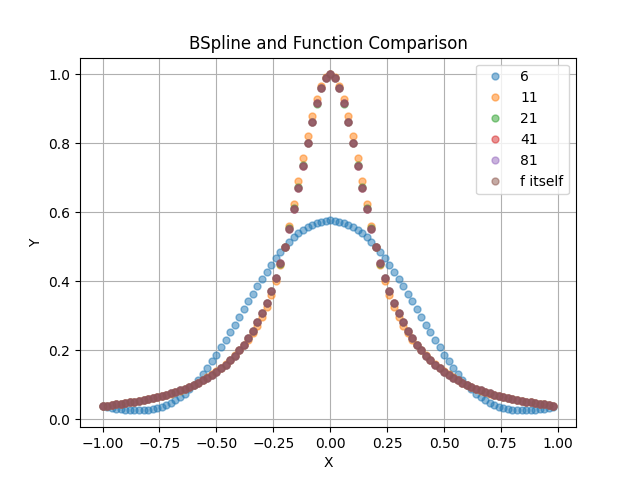
\includegraphics{../figure/ppForm_runge.png} 
        \caption{ppForm\_runge} 
    \end{figure}
    \begin{figure}[H] 
        \centering
        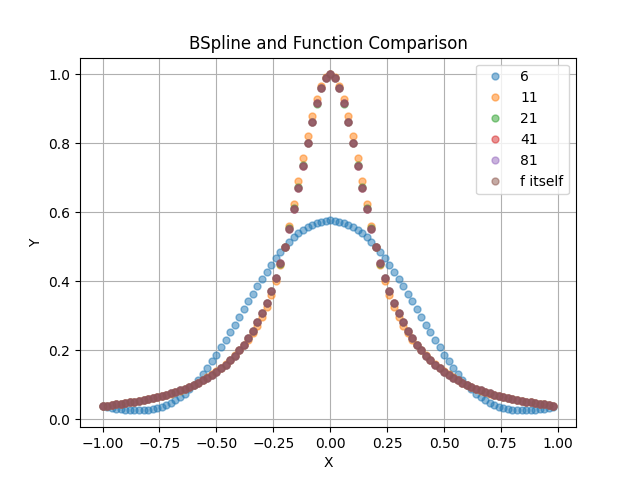
\includegraphics{../figure/BSpline_runge.png} 
        \caption{BSpline\_runge} 
    \end{figure}
    It can be seen that splines can effectively solve the Runge phenomenon.
    
    Plot the curve of maximum error variation:
    \begin{figure}[H] 
        \centering
        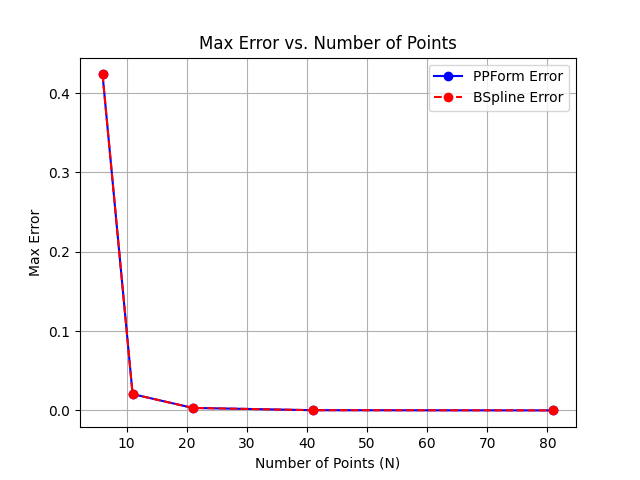
\includegraphics{../figure/max_error_plot.png} 
        \caption{max\_error\_plot} 
    \end{figure}
    
\section*{Problem C}
    The test file is located in \texttt{src/problems\_in\_chapter3/ProblemC.cpp}.
    The problem requires the use of Theorem 3.57 and Theorem 3.58 from the book.
    Therefore, in the path \texttt{src/problems\_1\_7/problem3/BSpline\_2\_3\_complete.hpp},
    two BSpline\_uniform\_23 and BSpline\_uniform\_12 are specifically implemented using the two theorems from the book.
    The accepted JSON templates are as follows:
    \begin{verbatim}
        {
            {"data points", knots1},
            {"values",value1},
            {"diff_values",{double(10)/(26*26),-double(10)/(26*26)}},
            {"range", {
                {"end", 5},
                {"begin", -5}
            }}
        };
    
        {
            {"data points", knots2},
            {"values",value2},
            {"boundary_values",{f(-5),f(5)}},
            {"range", {
                {"end", 4.5},
                {"begin", -4.5}
            }}
        }
    \end{verbatim}
    The implementation idea is the same as in the book, constructing the same coefficient matrix, solving for coefficients, and substituting.
    The part of calculating B-spline values calls the previous base class BSpline content, constructing the function value table.
    Running results:
    \begin{figure}[H] 
        \centering
        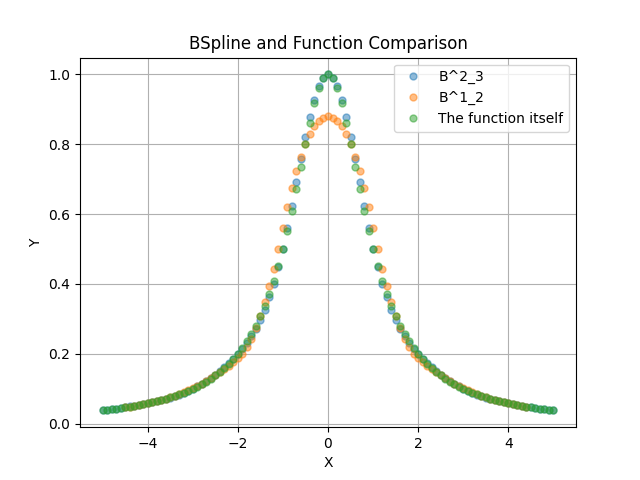
\includegraphics{../figure/Pc.png} 
        \caption{Pc} 
    \end{figure}
    
    \section*{Problem D}
    The test file is located in \texttt{src/problems\_in\_chapter3/ProblemD.cpp}.
    Similar to C, calculate the error and output.
    \begin{figure}[H] 
        \centering
        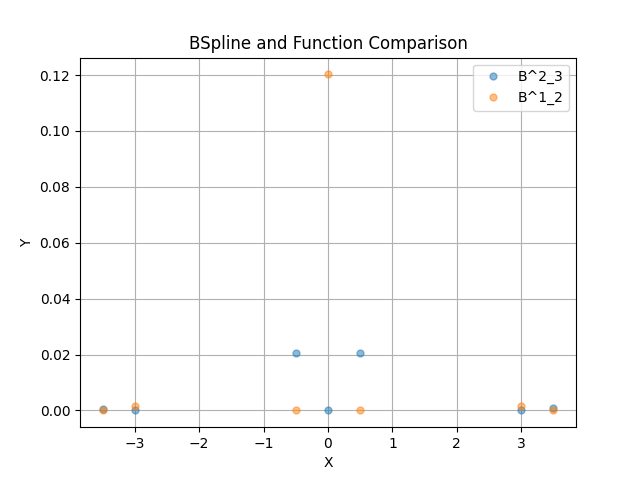
\includegraphics{../figure/Pd.png} 
        \caption{Pd} 
    \end{figure}
    Some points are on the interpolation points, so the output function values are almost the same as the original function values.
    It can be seen that the interpolation effect of $S^2_3$ is better.
    
\section*{Problem E}
    The test file is located in \texttt{src/problems\_in\_chapter3/ProblemE.cpp}.
    In Problem 6, these two parameterization methods have been introduced.
    Here, three functions are defined to take a certain number of control points, construct JSON, and transmit to BSpline fitting and ppForm fitting, each with two parameterization methods.
    \begin{verbatim}
        string str1 = "equal", str2 = "Chord";
        curve_fitting_p pe1(j1, str1), pe2(j2, str1), pe3(j3, str1);
        curve_fitting_B be1(j1, str1), be2(j2, str1), be3(j3, str1);
        curve_fitting_p pc1(j1, str2), pc2(j2, str2), pc3(j3, str2);
        curve_fitting_B bc1(j1, str2), bc2(j2, str2), bc3(j3, str2);
    \end{verbatim}
    Plot points and draw, and use the function to predict whether there is self-intersection:
    (note: There are four curves on the image, and the program also has four outputs, but the BSpline output is the same as ppForm, causing the image to be covered)
    When taking 10 control points:
    \begin{figure}[H] 
        \centering
        \includegraphics[width=0.5\textwidth]{../figure/PE_10.png} 
        \caption{PE\_10} 
    \end{figure}
    Function output results:
    1, 3 self-intersect, 2 no self-intersection\\
    When taking 40 control points:
    \begin{figure}[H] 
        \centering
        \includegraphics[width=0.5\textwidth]{../figure/PE_40.png} 
        \caption{PE\_40} 
    \end{figure}
    Function output results:
    1, 3 self-intersect, 2 no self-intersection\\
    When taking 160 control points:
    \begin{figure}[H] 
        \centering
        \includegraphics[width=0.5\textwidth]{../figure/PE_160.png} 
        \caption{PE\_160} 
    \end{figure}
    Function output results:
    1, 3 self-intersect, 2 no self-intersection\\
    It can be seen that equal division has high versatility, and cumulative chord length is more suitable for situations where higher precision is required for some intervals.
    
\section*{Problem F}
    The test file directory is \texttt{src/problems\_in\_chapter3/ProblemF.cpp}.
    Plot truncated power functions.
    \begin{verbatim}
        double truncate(double x,int order){
            if(x>0) return pow(x,order);
            return 0;
        }
        void test_truncate(double t, string file_name,double begin,double end){
            ofstream outfile(file_name, ios::trunc);
            for (double x = begin; x <= end; x+=(end-begin)/100) outfile << x << " " << truncate(t-x,1) << endl;
            outfile << "#END# " <<"n=1"<< endl;
            for (double x = begin; x <= end; x+=(end-begin)/100) outfile << x << " " << truncate(t-x,2) << endl;
            outfile << "#END# " <<"n=2"<< endl;
        }
    \end{verbatim}
    The output result is
    \begin{figure}[H] 
        \centering
        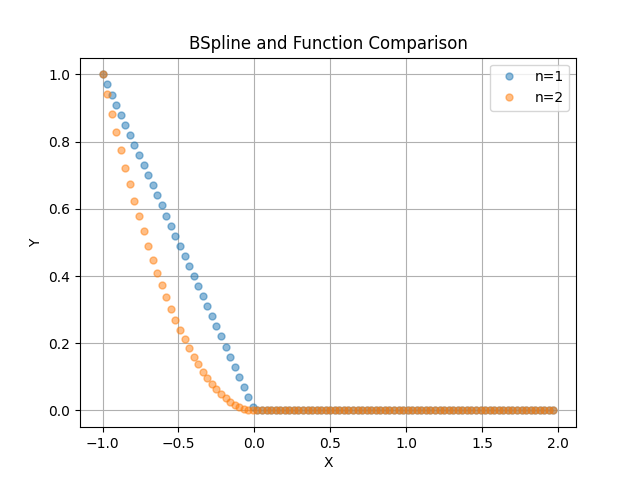
\includegraphics{../figure/PF_fig1.png}
    \caption{PF\_fig1} 
    \end{figure}

Calculate the function values at different positions for each x, and mark the positions.
\begin{verbatim}
void divide_truncate(vector<double> t,string file_name,int order){
        if(t.size()<order+2){
            cerr<<"invalid knot"<<endl;
            throw "invalid knot";
        }
        ofstream outfile(file_name, ios::trunc);
        int i=0;
        for (double x = t[0]-1; x <= t[t.size()-1]; x+=0.1)
        {
            vector<double> value(order+2);
            for (i = 0; i < order+2; i++)
            {
                value[i]=truncate(t[i]-x,order);
                outfile<<"t_{"<<i-1<<","<<0<<"}"<< x << " " << value[i] << endl;
            }
            for (size_t layer = 1; layer < order+2; layer++)
            {
                for (i = layer; i < order+2; i++)
                    {
                    value[i]=(value[i]-value[i-1])/(t[i]-t[i-1]);
                    outfile<<"t_{"<<i-1<<","<<layer<<"}"<< x << " " << value[i] << endl;
                    }
            }
        }
    }
\end{verbatim}
Draw
\begin{figure}[H]
\centering
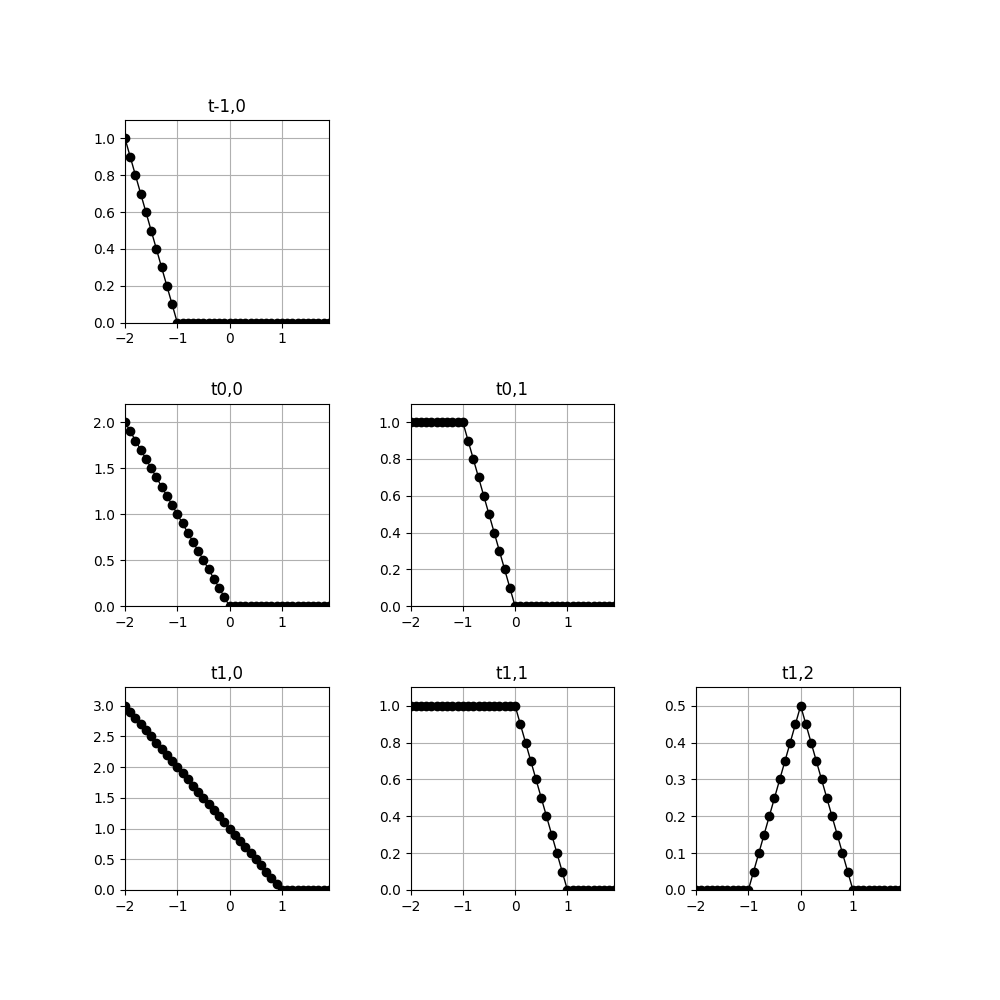
\includegraphics[width=0.5\textwidth]{../figure/PF_fig2.png}
\caption{PF\_fig2}
\end{figure}
\begin{figure}[H]
\centering
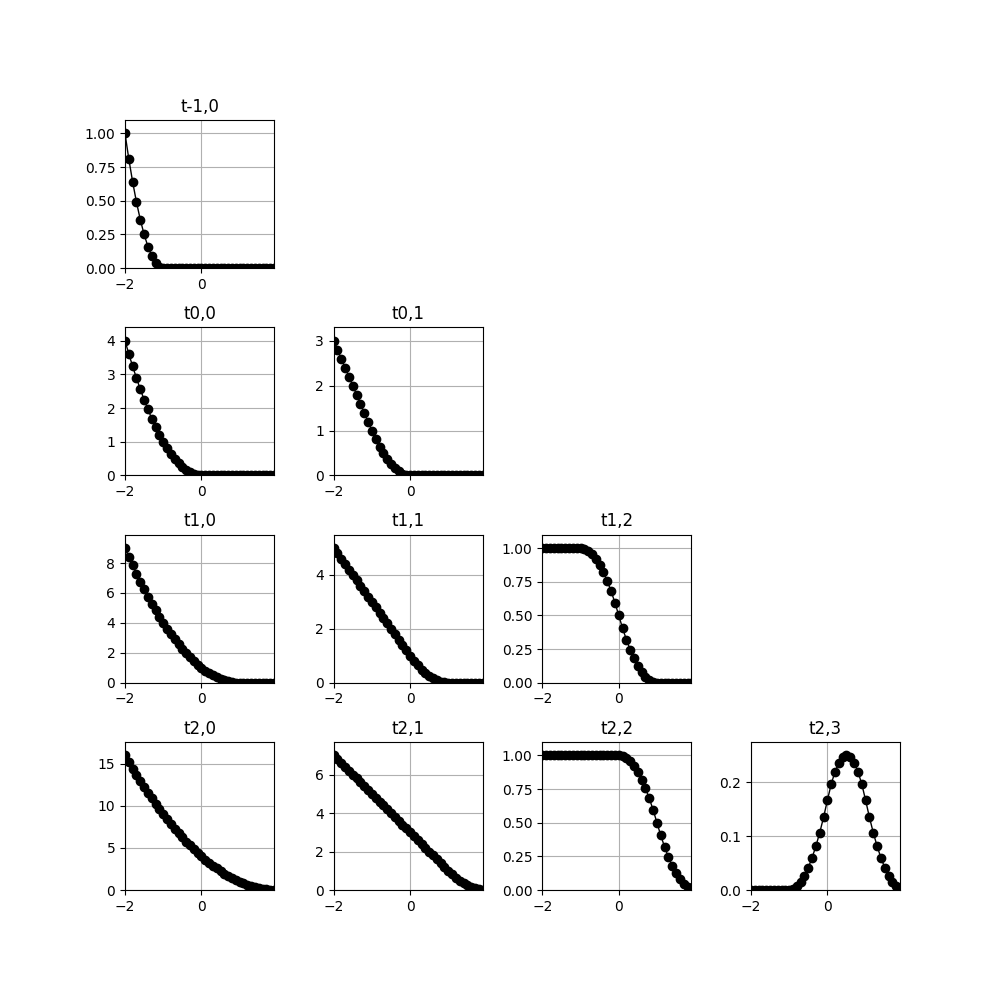
\includegraphics[width=0.5\textwidth]{../figure/PF_fig3.png}
\caption{PF\_fig3}
\end{figure}


\section*{Bonus 1}
Using jsoncpp:
The program accepts JSON as input and can freely combine various equations and assign various boundary conditions, accepting specified ranges, arbitrary order, nodes, and dimensions.

\section*{Bonus 2}
Implemented arbitrary-order ppForm and BSpline.
Also supports free combination of any boundary conditions.

\section*{Bonus 3}
Code location: \texttt{src/bonus/convergencerate.cpp}
Here, sin(x) is used as a test case.
The boundary condition is set to not\_a\_knot.
\begin{verbatim}
    j={
        {"dimension",1},
        {"order", 3},
        {"boundary condition", {
            {"values", {
                num,
                orders,
                y
            }},
            {"exists",{1,n-2}}
        }},
        {"data points", x},
        {"range", {
            {"end", domain.second},
            {"begin", domain.first}
        }}
    }
\end{verbatim}
Using BSpline:
\begin{verbatim}
    n           Max Error   Convergence Order
    --------------------------------------------------
             4           0.0436158                   -
             8          0.00051178            5.246420
            16         1.16408e-05            4.964147
            32         3.10621e-07            4.991757
            64          1.6027e-08            4.180091
           128         9.71338e-10            3.998779
           256         5.98314e-11            3.998333
\end{verbatim}
Using ppForm:
\begin{verbatim}
                n           Max Error   Convergence Order
    --------------------------------------------------
         4           0.0436158                   -
         8          0.00051178            5.246420
        16         1.16408e-05            4.964147
        32         3.10621e-07            4.991757
        64          1.6027e-08            4.180091
       128         9.71337e-10            3.998779
       256         5.98317e-11            3.998325
\end{verbatim}
It can be seen that as the number of points increases, the convergence order approaches 4.

\section*{Bonus 4}
Designed more functions for plane fitting.
\begin{figure}[H] 
    \centering
    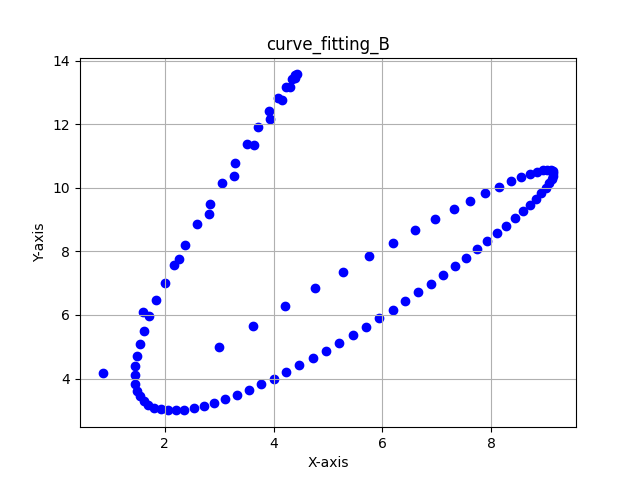
\includegraphics{../figure/curve_fitting_B_1.png} 
    \caption{curve\_fitting\_B\_1} 
\end{figure}
\begin{figure}[H] 
    \centering
    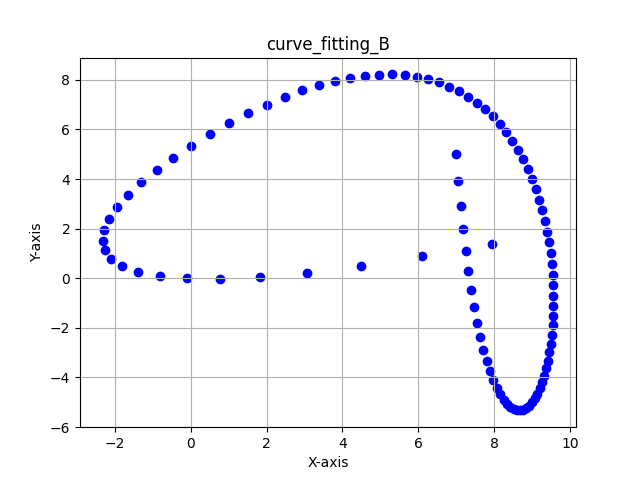
\includegraphics{../figure/curve_fitting_B_2.png} 
    \caption{curve\_fitting\_B\_2} 
\end{figure}
\begin{figure}[H] 
    \centering
    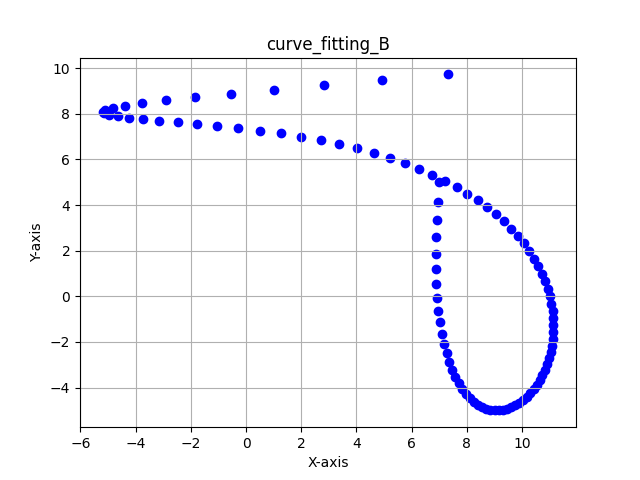
\includegraphics{../figure/curve_fitting_B_3.png} 
    \caption{curve\_fitting\_B\_3} 
\end{figure}

\section*{Bonus 5}
Designed a program to determine whether there is self-intersection.
Function location: \texttt{src/bonus/intersect.hpp}
The function
\texttt{bool detect\_intersect(json j)}
The JSON format requirement is the same as Problem 6.
Given control points, use splines for fitting first.
Then take points uniformly and bring them into the spline to get a series of point sets.
\begin{verbatim}
    for (int i = 0; i <= num_samples; ++i) {
        double t = std::max(std::min(start + i * (end - start) / num_samples, end), start);
        auto value = B.get_value(t);
        points.push_back({value});
    }
\end{verbatim}
These adjacent points are connected to form small line segments, and these small line segments are combined in pairs to determine if they intersect.
As the number of points increases, the judgment accuracy is higher.
\begin{verbatim}
    bool segments_intersect_nd(const PointND& p1, const PointND& q1, const PointND& p2, const PointND& q2) {
        const double epsilon = 1e-9;
        auto d1 = subtract(q1.coords, p1.coords);
        auto d2 = subtract(q2.coords, p2.coords);
        auto r = subtract(p1.coords, p2.coords);
        double a = dot(d1, d1);
        double b = dot(d1, d2);
        double c = dot(d2, d2);
        double d = dot(d1, r);
        double e = dot(d2, r);
        double denom = a * c - b * b;
        double t, s;
        if (fabs(denom) > epsilon) { // not parallel
            t = (b * e - c * d) / denom;
            s = (a * e - b * d) / denom;   
            if (t < 0 || t > 1 || s < 0 || s > 1) return false;
        } else { // parallel
            double d1_proj = dot(d1, r);
            double d2_proj = dot(d2, subtract(q1.coords, p2.coords));
            if (fabs(d1_proj) > epsilon || fabs(d2_proj) > epsilon) return false;
        }
        // If the distance is less than the threshold, it is considered to intersect
        auto p1_proj = subtract(p1.coords, subtract(d1, d2));
        double distance = dot(p1_proj, p1_proj);
        return distance < epsilon;
    }
\end{verbatim}
Note to avoid comparing adjacent, shared vertex small line segments.
Tested on the samples in Problem E and Problem 7, both are correct.




\section*{ \center{\normalsize {Acknowledgement}} }
    Use GPT-4 for quick template transformation, and use Kimi AI to correct English grammar.
    
\end{document}
    

